% introduce CTMC 
\begin{frame}
\frametitle{Modelling Imbalance}

\end{frame}

% introduce nFPC calibration   
\begin{frame}
\frametitle{Incorporating Price Change}
Next, consider a two-dimensional CTMC $Z(t)$ that jointly models imbalance bin $\rho(t)$ and price change $\Delta S(t)$, where 
\[ \rho(t) \in \lbrace 1,2,\dots,\#_{bins} \rbrace \]
is the bin corresponding to imbalance averaged over the interval $[t-\Delta t_I, t]$, and
\[ \Delta S(t) = \sgn(S(t+\Delta t_S)-S(t)) \in \lbrace -1, 0, 1 \rbrace \]  
is the \emph{sign} of the change in midprice of the \emph{future} time interval $\Delta t_S$.

\adjustimage{max size=\textwidth}{frames/figs/timewindows.pdf}
\end{frame}

% P matrix.
\begin{frame}
\frametitle{Transition Matrix}
Using MLE, we obtain a generator matrix $\mat{G}$ for the CTMC. The transition matrix over a step of size $\Delta t_I$ is given by
\[ \mat{P}(\Delta t_I) = [p_{ij}(\Delta t_I)] = e^{\mat{G} \Delta t_I} \]
called our \emph{one-step transition probability matrix}. Matrix entries give the probability of transition from one (imbalance, price change) pair to another over the time interval $\Delta t_I$. This can be written semantically as
\[ p_{ij} = \mathbb{P}\left[ \varphi( \rho_\text{curr}, \Delta S_\text{future}) = j \; | \; \varphi( \rho_\text{prev}, \Delta S_\text{curr} ) = i \right] \]
\end{frame}

% ... Bayes transform into Q matrix ...
\begin{frame}
\frametitle{Predicting Future Price Change}
Using Bayes' Rule, we can transform the $\mat{P}$ matrix to 
\[ \mathbb{P}\left[ \Delta S_\text{future} = j \; | \; B, \rho_\text{curr} = i \right] = \dfrac{\mathbb{P}\left[ \rho_\text{curr} = i, \Delta S_\text{future} = j \; | \; B \right]}{\mathbb{P}\left[ \rho_\text{curr} = i \; | \; B \right]} \]
This allows us to predict future price moves.
\vspace{\baselineskip}
We'll call the collection of these probabilities the $\mat{Q}$ matrix.
\end{frame}

% show sample Q. 
\begin{frame}
\frametitle{Predicting Future Price Change}
Sample $\mat{Q}$ matrix.
\begin{table}%
\ra{1.2}%
\begin{adjustbox}{width=\textwidth}
\begin{tabular}{@{} r@{\hskip 1cm} *{9}{r} @{}}%
\toprule
& \multicolumn{3}{c}{$\Delta S_\text{curr} < 0$} & \multicolumn{3}{c}{$\Delta S_\text{curr} = 0$} & \multicolumn{3}{c}{$\Delta S_\text{curr} > 0$} \\
\cmidrule(lr){2-4} \cmidrule(lr){5-7} \cmidrule(lr){8-10}
\multicolumn{2}{r}{$\rho_{curr} = 1$} & 2 & 3 & 1 & 2 & 3 & 1 & 2 & 3 \\
\midrule
\multicolumn{10}{l}{$\Delta S_\text{future} < 0$} \\
$\hphantom{abcd}\rho_\text{prev} = 1$ & \bf 0.53 & 0.15 & 0.12 & 0.05 & 0.10 & 0.14 & 0.08 & 0.13 & 0.14 \\
$\rho_\text{prev} = 2$ & 0.10 & \bf 0.58 & 0.14 & 0.07 & 0.04 & 0.10 & 0.13 & 0.06 & 0.12 \\
$\rho_\text{prev} = 3$ & 0.08 & 0.12 & \bf 0.52 & 0.09 & 0.06 & 0.03 & 0.11 & 0.10 & 0.05 \\[0.6ex]
\multicolumn{10}{l}{$\Delta S_\text{future} = 0$} \\
$\rho_\text{prev} = 1$ & 0.41 & 0.75 & 0.78 & \bf 0.91 & 0.84 & 0.79 & 0.42 & 0.79 & 0.77 \\
$\rho_\text{prev} = 2$ & 0.79 & 0.36 & 0.71 & 0.83 & \bf 0.92 & 0.82 & 0.75 & 0.37 & 0.78 \\
$\rho_\text{prev} = 3$ & 0.79 & 0.74 & 0.40 & 0.81 & 0.83 & \bf 0.91 & 0.70 & 0.76 & 0.39 \\[0.6ex]
\multicolumn{10}{l}{$\Delta S_\text{future} > 0$} \\
$\rho_\text{prev} = 1$ & 0.06 & 0.10 & 0.09 & 0.04 & 0.06 & 0.07 & \bf 0.50 & 0.09 & 0.09 \\
$\rho_\text{prev} = 2$ & 0.10 & 0.06 & 0.15 & 0.10 & 0.04 & 0.08 & 0.12 & \bf 0.57 & 0.10 \\
$\rho_\text{prev} = 3$ & 0.13 & 0.14 & 0.08 & 0.10 & 0.11 & 0.05 & 0.19 & 0.14 & \bf 0.56 \\
\bottomrule
\end{tabular}%
\end{adjustbox}%
\end{table}%
\end{frame}

% present Naive strategies 1-3
\begin{frame}
\frametitle{Trading Strategies Informed by the $\mat{Q}$ Matrix}
\begin{itemize}
\item[Naive] Use market orders to buy (sell) if price is predicted to move up (down).
\item[Naive+] Post at-the-touch limit orders when zero price change is predicted.
\item[Naive++] Post a limit order to buy (sell) is price is predicted to move up (down).
\end{itemize}
\end{frame}

\begin{frame}
\frametitle{Calibration of Naive Trading Strategies}
Need to select:
\begin{itemize}
\item price change observation period $\Delta t_S$
\item imbalance averaging period $\Delta t_I$
\item number of imbalance bins $\#_{bins}$
\end{itemize}
Calibration done on the first day of the trading year, same parameters used for all days.

Brute-force search of parameter space, using max Sharpe ratio criterion, found that $\Delta t_S = \Delta t_I = 1 sec$, and $\#_{bins} = 4$
\end{frame}

% present plots
\begin{frame}
\frametitle{Results of Naive Trading Strategies}
\begin{figure}%
\centering%
\subfloat{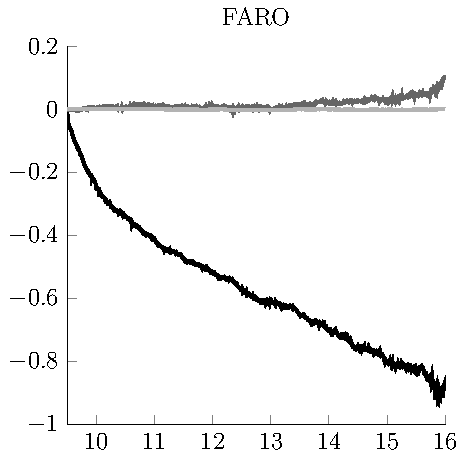
\includegraphics[height=.3\textwidth, width=.35\textwidth]{frames/figs/FARO_naive_strat_comp.pdf}}\quad
\subfloat{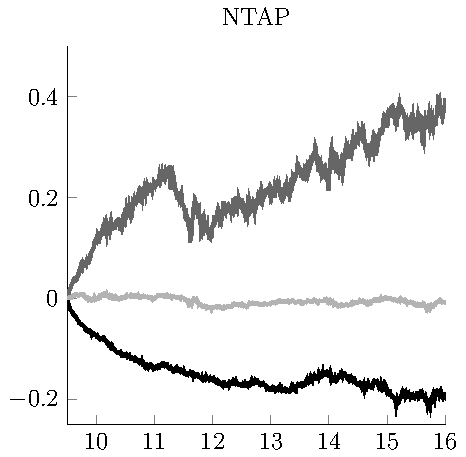
\includegraphics[height=.3\textwidth, width=.35\textwidth]{frames/figs/NTAP_naive_strat_comp.pdf}}\\
\subfloat{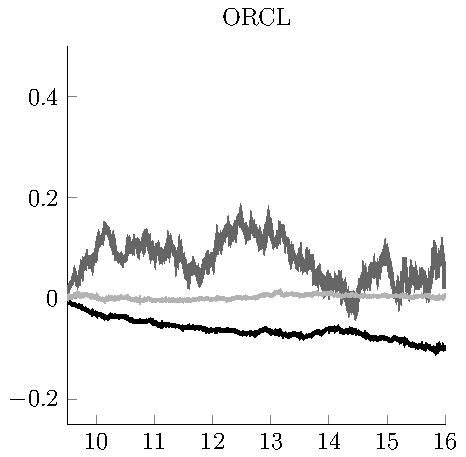
\includegraphics[height=.3\textwidth, width=.35\textwidth]{frames/figs/ORCL_naive_strat_comp.pdf}}\quad
\subfloat{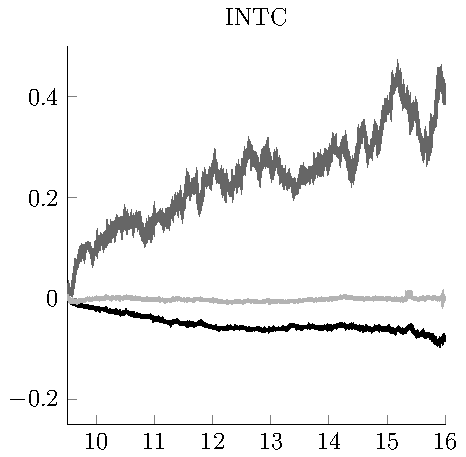
\includegraphics[height=.3\textwidth, width=.35\textwidth]{frames/figs/INTC_naive_strat_comp.pdf}}\\
%
\leavevmode\smash{\makebox[0pt]{\hspace{2em}% HORIZONTAL POSITION           
  \rotatebox[origin=l]{90}{\hspace{3em}% VERTICAL POSITION
	Normalized Profit and Loss (P\&L)}%
}}\hspace{0pt plus 1filll}\null%

Time (h)

\vspace{1cm}%
\subfloat{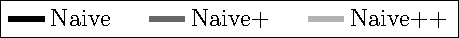
\includegraphics[scale=1]{frames/figs/naivestratlegend.pdf}}%
\end{figure}

\end{frame}

% talk about calibration and failures
\begin{frame}
\frametitle{Conclusions from Naive Trading Strategies}
{\bf Why is the Naive strategy producing, on average, normalized losses?}
\begin{itemize}
\item Backtest is out-of-sample; evidence to reject time-homogeneity
\item Calibration is done on first trading day; likely nonrepresentative of trading activity
\item Price change probability matrix $\mat{Q}$ obtained using midprices, ignoring bid-ask spread; $\sgn(\Delta S)$ may be insufficient for create profit, especially on \texttt{FARO}
\end{itemize}
\end{frame}

\begin{frame}
\frametitle{Conclusions from Naive Trading Strategies}
{\bf Why do the Naive+ and Naive++ strategies outperform the Naive strategy?}
\begin{itemize}
\item LOs vs MOs means different transaction price is being used (only MO loses value)
\item Naive only executes when predicting non-zero price change
\begin{itemize}
\item Only sign, not magnitude
\item Only \emph{if one was already seen}
\end{itemize}
\end{itemize}
\end{frame}
